\documentclass[]{article}
\usepackage[margin=1in]{geometry}
\usepackage{graphicx}

\begin{document}

\title{Progress Report}
\author{Matt Smith}
\date{\today}
\maketitle

\section{Project Description}

This project, ultimately, aims to provide a simulation of individuals attempting to give up smoking in the situation of a social network. In particular, focus is given to how the network manipulates their behaviour and whether some social organisations and constructs are more suited to triggering the breaking of the smoking habit. To analyse this, a model of both a human and a social network will be created, through which a given period of time can be simulated - the result of this being data that can be analysed to find the previously mentioned social conditions conducive to give up smoking.

\section{Progress Summary}

On the whole, the project continued to be consistent with the project specification, insofar as rather than large changes having to be made, specific details and implementation methods are now known, and there is a greater understanding about the theoretical basis of the models. No development towards the final model has been started - to date, experimental code has been written as proof-of-concept programs to examine different approaches. These pieces of work will, however, form the basis for parts of the final model.

\section{Model Research Progress}

\subsection{Human Representation}

As modelling a human (also referred to as a \emph{node}) in general is a difficult task, the scope of the project can be reduced significantly by ensuring that only aspects of human behaviour related to the analysis of smoking are used. Furthermore, some assumptions about the way in which nodes behave have to be made to prevent the project encompassing a large part of sociological and psychological theory. Due to this, it has been decided that the human behaviour will be represented in a probabilistic manner - the reasons for this are twofold. First, is that it provides a simple method of recreating some facets of actions, for example a person could rate, on a scale of one to ten, how likely they are to start smoking in the next few days. Although this is not necessarily an accurate measure, it is enough for a simplistic representation. Example attributes include:

\begin{itemize}
\item \emph{Susceptibility to peer-pressure} - peer-pressure may over-ride other considerations
\item \emph{Likeliness to smoke} - humans may have an internal opinion on smoking that guides them.
\item \emph{Willpower} - how likely they are to continue their giving-up effort.
\item \emph{Number of Cigarettes Per Day} - a higher number may make giving up harder.
\item \emph{Ability to Influence} - hub nodes may be influential, and as such be powerful.
\end{itemize}

Some attributes, however, cannot be representing by probabilities. These include items such as how many cigarettes someone smokes, whether someone smokes at all and how likely they are to reach out beyond their local network.

Representing this series of decisions will be done through the use of a decision tree - a series of choices that the person can make, leading them to some state consisting of a collection of attribute values. The key advantages of this are that it allows a fixed number of choices per tick, with the ability to structure the choices (for example, important ones at the top). The structure and content of this tree is largely a developmental matter and needs to be tuned over time, but a concept tree can be seen in figure \ref{fig:Sample decision tree}.


\begin{figure}
	\centering
		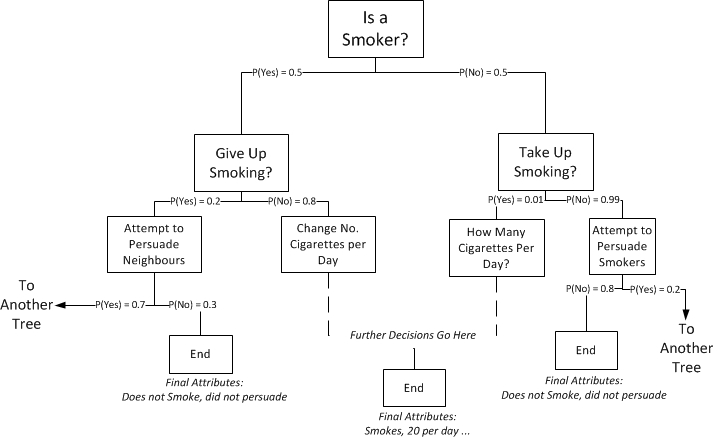
\includegraphics[width=0.80\textwidth]{sdt.jpg}
	\caption{Example Decision Tree}
	\label{fig:Sample decision tree}
\end{figure}


In terms of the model-at-large, it is important for the network to be able to reconfigure itself over time, due to the notion of homophily \cite{USN} - this is the concept of people with similar interests since people move towards to others with similar interests whilst at the same time, friends will develop similar interests within the relationship. This leads to a split between influence and reconfiguration. The former is a major focus of this project, since understanding how the influence flows around a social network is key to concluding how the network impacts behaviour. 

Up to this point, only the human as a single entity has been considered - to model effects of interacting with others, influence must be modelled. In the current plans, the \emph{Linear Threshold} model will be used to implement influence - it is based upon the concept of the number of neighbours for a given node holding an attribute or performing an action will increase the chance of the node also taking on that attribute/performing the action. In addition, the previously mentioned decision tree can either incorporate or have a standalone tree for the impact of incoming influence from surrounding nodes. Once more, this will be done probabilistically, where the edge weights either dampen or emphasise the influence passing through them (see below). 

Reconfiguration is also important, but is much harder to accurately model - to maintain a reasonable project scope, this will not be as formal as an implementation. It is likely that a decision tree will be created that will choose and negotiate relationships with other nodes, with the aim of building a model that will emulate the previously mentioned concept of homophily.

To further the attempt of emulating human actions, the system will have `Acts of God', where random behaviours will be introduced with a very small probability. This will be tuned to have the impression of subtly unsettle the network and prevent it falling into equilibrium for long periods of time, whilst also attempting to simulate the human behaviour of occasionally acting out of character. \emph{More research to come here.}

In terms of the items that propagate, attributes are a particular focus - the idea of others affecting your choices is key to this process. Example attributes that would propagate are whether someone smokes, and the number of cigarettes someone smokers, per day - if person's friend smokes heavily, then the person may increase to allow them to spend more time with their friend. As such, the probabilities used in the decision trees will be manipulated by the nodes connected to a given person. The overall aim is that these manipulations will represent the overt and subconscious actions of others that encourage someone to choose a particular action.

\subsection{Network Representation}
One of the key factors in the success of this project was to be able to generate a realistic social network, as without this, the model would be unable to produce meaningful results. To date, two methods have come out as useful in the research - \emph{small-world} and \emph{scale-free}, the latter being a type of \emph{preferential attachment} network.

Small-world networks are created using the Watts \& Strogatz model \cite{WSTech}, and produce graphs similar to the one shown below in figure \ref{fig:small-world}. In general, the method uses a degree averaging technique to give all members in the graph roughly the same number of edges. As implied by the name, this method is strongly related to the idea that most people know each other, or if not directly, through a small number of connections - as such, this is not entirely useful to this project as it is difficult to realistically model the environment of larger groups of people. 

\begin{figure}
	\centering
		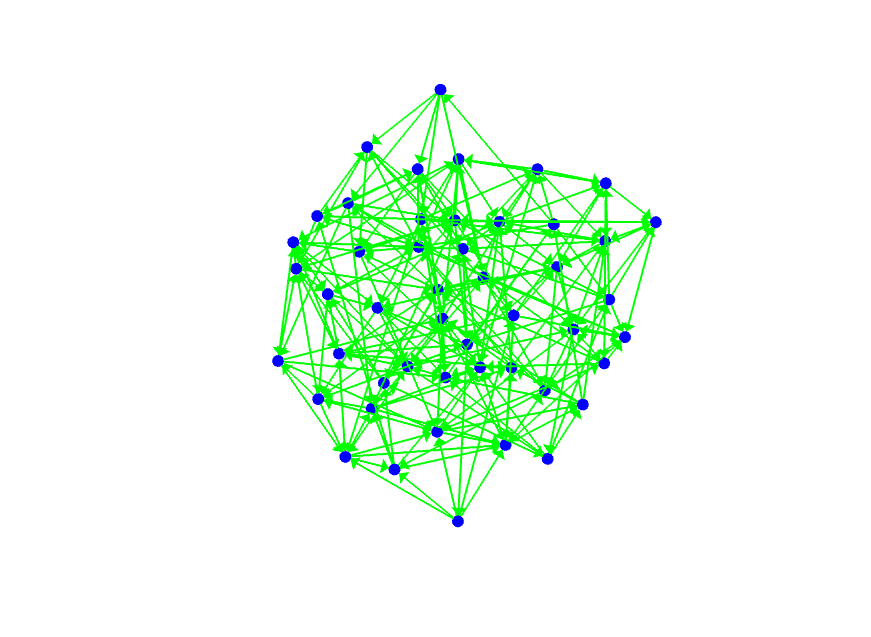
\includegraphics[width=0.80\textwidth]{small-world.png}
	\caption{Small-World Network - 50 nodes, $\beta$ = 0.5, K = 10 - Layout: Fruchterman-Reingold Algorithm}
	\label{fig:small-world}
\end{figure}


In a larger graph, it is highly unlikely that most people know each other within a few connections, so the creation of a scale-free network (using the \emph{Barab\'{a}si}-\emph{Albert} model \cite{BAMod}) succeeds here. This uses a \emph{preferential attachment} method - ``the rich get richer'' - to generate networks which instead have a number of `hub' nodes, similar to popular figures in friendship circles. Additionally, the graph is significantly less connected, resulting in a seemingly more realistic network. As can be seen in figure \ref{fig:scale-free1}, a basic scale-free graph of the same number of nodes exhibits features such as `hubs' and groups of nodes. Furthermore, when increased to 250 nodes(fig. \ref{fig:scale-free2}), these features are emphasised. With some modification of this algorithm, networks produced should approach realistic social networks. Note that there are a lot of outliers - this would have to be accounted for in modifications, for example by removing a certain percentage of them.

\begin{figure}
	\centering
		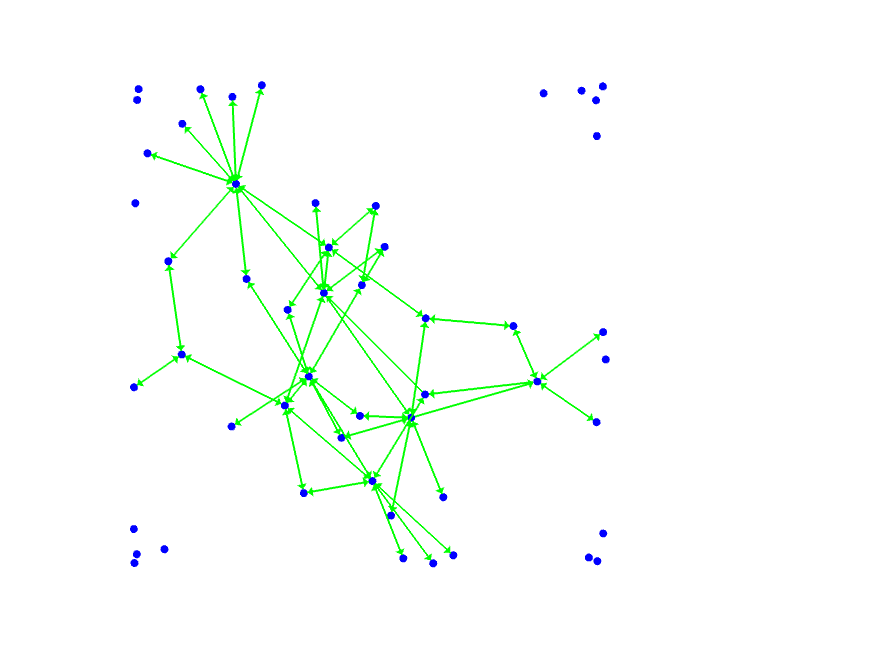
\includegraphics[width=0.80\textwidth]{scale-free1.png}
	\caption{Scale-Free Network - 50 nodes, starting with 4 vertices, 3 edges - Layout: Fruchterman-Reingold Algorithm}
	\label{fig:scale-free1}
\end{figure}

\begin{figure}
	\centering
		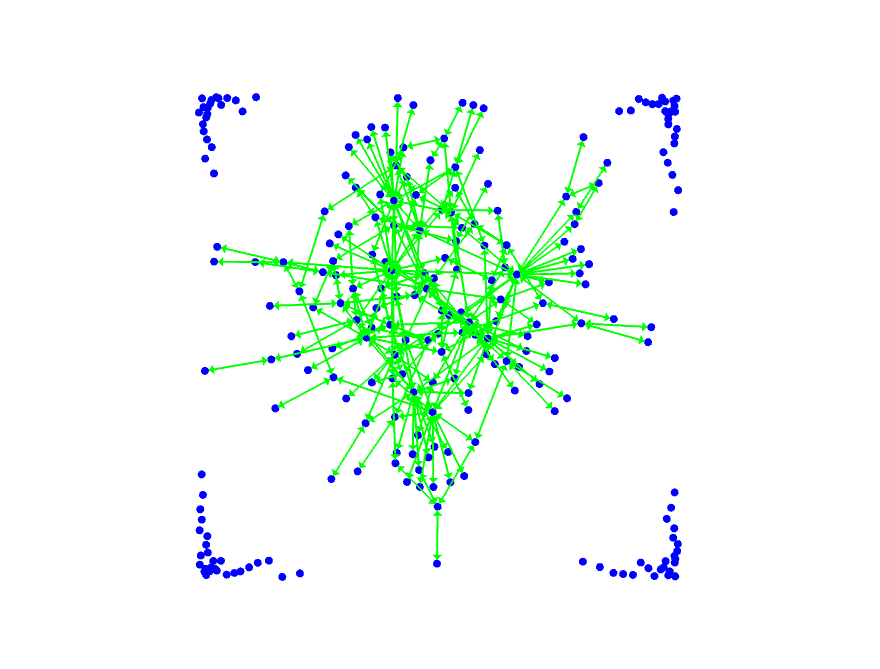
\includegraphics[width=0.80\textwidth]{scale-free2.png}
	\caption{Scale-Free Network - 250 nodes, starting with 4 vertices, 3 edges - Layout: Fruchterman-Reingold Algorithm}
	\label{fig:scale-free2}
\end{figure}

\emph{Metrics relating to small-world vs scale free will go here, e.g. network diameter, average distance and more.}
\emph{Further details about how realistic these networks are will be included here.}

Alongside the generated networks, sampled networks will also be gathered - by combining these with a set of generated networks, developmental models of components such as the decision tree can be tuned with the ability to reproduce model behaviour. Working from this, larger data sets can be both gathered from real datasets and computer-generated to provide a wide range of networks usable in the final analysis. 

Moving from the whole network to individual edges, relationships in a social network map well to a directed graph. This is because relationships are not necessarily symmetric - assuming they are removes the concept of role-models, an important feature of social networks, and also blocks another key concept,  that of different people being influenced by others to a different degree. 

Using this idea, it has been decided that edge-weight should represent the `influence factor' of that relationship - if node A has an edge of weight 0.5 to node B, then any behaviours that traverse this edge will only do so with an impact of half the original. Firstly, this reinforces the idea of role-models (a person is highly influenced by another, but the other is not necessarily influenced, or even knows, the first). It also provides a more realistic approximation of how a friendship works, since although friends, one person may think more of the other and as such tend to be influenced more easily by them. Values between 0 and 1 will be used here to maintain the probabilistic approach.

\subsection{User Features}

There are two main user features that are to be included in the project, to date. The first is the generation of networks based on loose statistics - this, when combined with both the previously mentioned network generators and the human model, will be a relatively trivial interface between the initialisation of the simulation environment and the user, so should cause no problems in the development phase. 

The other feature is the ability to parse and export existing graphs - again, as mentioned above, work has gone into parsing datasets and outputting them as \emph{GraphML} - to work this into the simulation setup should be relatively simple as it is based on code already written. A particularly useful feature would be to export the network to \emph{GraphML} at given simulation ticks, to allow for static analysis of the network at a given time. 

\subsection{Commercial Model Integration}

At this stage, it would not be suitable to consider whether the model will fit into a larger, commercial-level model as not enough development of the model itself has been completed. It should be noted, however, that up to now, there have been no issues that would appear to cause any problems. 

\subsection{Visualisation}

Along with simulating the human and network behaviour, it is important to be able to view snapshots of the model to understand what is happening. So far, this has come via two avenues - \emph{Gephi} and the \emph{Repast GUI}. Gephi is particularly useful when it comes to generating standalone networks for analysis - examples of this include inspecting algorithm-generated networks for realism and checking if a sampling method is working correctly, producing a reasonable graph. The \emph{Repast GUI} provides a similar service but is refreshed on each simulation tick. Due to this, the GUI effectively gives a live view of the network and how it is behaving - of course, this is has some more simplistic tools than \emph{Gephi}, so works in a complementary way.

\subsection{Analysis of Model}

Although final analysis methods are yet to be decided, great care has been taken to ensure that there is as larger range as tools as possible available for analysis, and as such stopping any implementation based restrictions on these tools. An example of this include building a \emph{GraphML} serialiser for \emph{JUNG} networks, to allow for \emph{Gephi}/\emph{Cytoscape} analysis of these graphs. Considering final analysis methods, statistical methods are likely to form the basis of comparing realistic models to the model produced as part of this project - this will provide a numerical approach to evaluating the `realism' of the networks and nodes involved.

\section{Timetable}
To be added.

\bibliographystyle{plain}
\bibliography{progRepBib}

\end{document}